\subsection{Interpreter Architecture}

\YIComment{Explain how interpreter works}

\begin{figure}[h]
    \centering
    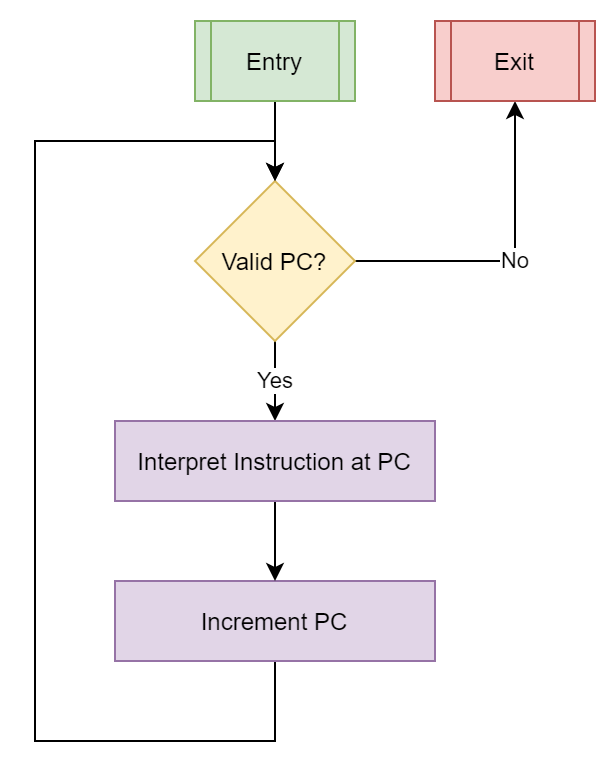
\includegraphics[width=0.5\linewidth]{diagrams/interpreter.png}
    \caption{Top level architecture of the interpreter emulator.}
    \label{figure:interpreter-arch}
\end{figure}

\subsubsection{Interpreter Core}

\YIComment{Do this}

\subsubsection{Register File}

\YIComment{Do this}

\subsubsection{Memory Map}
\label{section:interpreter-mem-map}

The memory map uses an associative model powered by an unordered hash table. This allows for the entire 32-bit address space to be emulated without requiring it to be pre-allocated, something that might prove difficult in a 32 bit process. The current implementation allows for $\mathcal{O}(1)$ read and write times. Despite this, the performance is substandard compared to a raw array due to the extra overhead and being less cache friendly.

After profiling, the \texttt{std::unordered\_map} originally used was found to be a bottleneck and thus was replaced with a 3rd party implementation Tessil/robin-map \cite{tessil-map, tessil-benchmark}.